%=============================================================================
%  AD_COURSEWORK_GROUP_X.tex  --  Advanced Derivatives coursework 2026-27
%  DRAFT.  All numbers, tables and figures are produced by
%  ad_coursework_code.py (run it first: it writes ./figures and ./tables).
%  Report (excluding cover page) must be at most 10 pages.
%=============================================================================
\documentclass[11pt,a4paper]{article}

\usepackage[T1]{fontenc}
\usepackage{lmodern}
\usepackage[utf8]{inputenc}
\usepackage[a4paper,margin=1.8cm,top=1.6cm,bottom=1.8cm]{geometry}
\usepackage{amsmath,amssymb}
\usepackage{graphicx}
\usepackage{xcolor}
\usepackage{xspace}
\usepackage{booktabs}
\usepackage{tabularx}
\usepackage{float}
\usepackage{caption}
\usepackage{listings}
\usepackage{enumitem}
\usepackage{hyperref}

\definecolor{linkblue}{RGB}{0,70,140}
\hypersetup{colorlinks=true, linkcolor=linkblue, urlcolor=linkblue,
            citecolor=linkblue}
\captionsetup{font=small,labelfont=bf,skip=4pt}
\setlength{\parskip}{3pt}
\setlength{\parindent}{0pt}
\setlist{itemsep=1pt,topsep=2pt}

\graphicspath{{figures/}}

\lstset{
  language=Python,
  basicstyle=\ttfamily\scriptsize,
  keywordstyle=\color{blue},
  commentstyle=\color{green!50!black},
  stringstyle=\color{red!70!black},
  showstringspaces=false,
  numbers=left,
  numberstyle=\tiny,
  stepnumber=1,
  frame=single,
  breaklines=true,
  aboveskip=4pt, belowskip=4pt,
  rangeprefix=\#\ [, rangesuffix=],
  includerangemarker=false
}
% \code{marker}{caption}: print the part of the code file between
% "# [marker_start]" and "# [marker_end]"
\newcommand{\code}[2]{%
  \lstinputlisting[linerange=#1_start-#1_end, caption={#2}]
  {ad_coursework_code.py}}
% \tab{file}{caption}{label}: a table produced by the code
\newcommand{\restab}[3]{%
  \begin{table}[H]\centering\footnotesize
  \caption{#2}\label{#3}
  \input{tables/#1.tex}
  \end{table}}
\newcommand{\fig}[4][0.82\textwidth]{%
  \begin{figure}[H]\centering
  \includegraphics[width=#1]{#2}
  \caption{#3}\label{#4}
  \end{figure}}
\renewcommand{\lstlistingname}{Code}

\begin{document}

%-----------------------------------------------------------------------------
%  COVER PAGE
%-----------------------------------------------------------------------------
\begin{titlepage}
\centering
\vspace*{1.5cm}

{\Large\bfseries EDHEC Business School}\\[3mm]
{\large M.Sc. in Financial Engineering}\\[18mm]

{\LARGE\bfseries Advanced Derivatives}\\[5mm]
{\LARGE Coursework Report}\\[6mm]
{\Large Academic Year 2026--27}\\[18mm]

{\Large\bfseries Group X}\\[10mm]

\begin{tabular}{@{}cll@{}}
\toprule
\# & Name & Student ID\\
\midrule
1 & Paolo Mastrogiacomo\hspace{2.5cm} & \hspace{3cm}\\
2 & \hspace{7cm} & \hspace{3cm}\\
3 & \hspace{7cm} & \hspace{3cm}\\
\bottomrule
\end{tabular}

\vfill
{\large Deadline: Tuesday 1 December 2026}\\[3mm]
{\normalsize Code: \texttt{ad\_coursework\_code.py} (all results reproducible,
fixed seeds)}
\vspace*{1.5cm}
\end{titlepage}

%=============================================================================
\section*{Question 1: Black-Scholes-Merton hedging}
%=============================================================================

\subsection*{1(a) Using the FinancePy library}
We call the analytic Black--Scholes functions in
\texttt{financepy.models.black\_scholes\_analytic} directly, with the option
type passed as an integer flag. In the current FinancePy release (1.1.x) these
functions are named \texttt{value}, \texttt{delta} and \texttt{gamma}; older
releases call them \texttt{bs\_value}, \texttt{bs\_delta},
\texttt{bs\_gamma}. The import handles both. For $S=K=100$, $r=4\%$,
$\sigma=20\%$, $T=1$ the put is worth $6.0040$, with delta $-0.3821$ and
gamma $0.01907$.
\code{imports}{Direct calls into the FinancePy model library.}

\subsection*{1(b) The \texttt{DeltaHedge} function}
At $t_0=0$ we receive the Black--Scholes premium $V_0$, buy $\Delta_0$ shares
(negative for a put) and put $B_0=V_0-\Delta_0S_0$ in the bank. On each of
the $NT$ dates the stock moves under the \emph{real-world} lognormal dynamics
with drift $\mu$, the bank account accrues $e^{r\Delta t}$, and we rebalance
to the new delta. Each rebalance is paid for out of the bank, so the
portfolio is self-financing. At expiry the replication error is
$\Delta_{T^-}S_T+B_T-(K-S_T)^+$. The realised variance is
$\frac1T\sum_i \ln^2(S_{i+1}/S_i)$. The assignment says the output has four
elements but lists five; we return all five.
\code{deltahedge}{\texttt{DeltaHedge}: self-financing delta hedge of a
European put.}

\subsection*{1(c) Running 10,000 paths}
\code{runpaths}{Wrapper that runs any hedging function over many paths and
returns a DataFrame.}

\subsection*{1(d) Hedging error versus terminal stock price}
\fig[0.68\textwidth]{q1_error_vs_ST.pdf}{Hedging error against $S(T)$ for $N=12,52,252$.
$S(0)=100$, $K=100$, $r=4\%$, $T=1$, $\sigma=\sigma_{\text{real}}=20\%$,
$\mu=8\%$, 10,000 paths per $N$.}{fig:q1-error}
The errors form a ``spindle'' centred on the strike. Paths that end far in
or far out of the money have small errors, because there the put's delta is
almost constant ($-1$ or $0$) and the hedge barely needs rebalancing. Paths
that end near $K=100$ have the largest errors, because that is where gamma
is highest and discrete rebalancing misses the most. The cloud shrinks
visibly as $N$ increases.

\subsection*{1(e) Mean and variance of the hedging error}
\restab{q1_moments}{Hedging error over 10,000 paths. ``Theory std.'' is the
Derman--Kamal approximation $\sqrt{\pi/4}\,\mathcal V\sigma/\sqrt N$, with
$\mathcal V$ the option's vega.}{tab:q1-moments}
The mean error is essentially zero, so the hedge is unbiased: the premium
is exactly enough to finance the replication. The variance falls roughly in
proportion to $1/N$: going from monthly to daily hedging cuts the standard
deviation from $1.95$ to $0.43$, about a third of the premium down to
$7\%$ of it. The simulated standard deviations match the Derman--Kamal
approximation almost exactly.

\subsection*{1(f)--(g) Realised volatility, average gamma and the replication error}
\begin{figure}[H]
\begin{minipage}[t]{0.49\textwidth}\centering
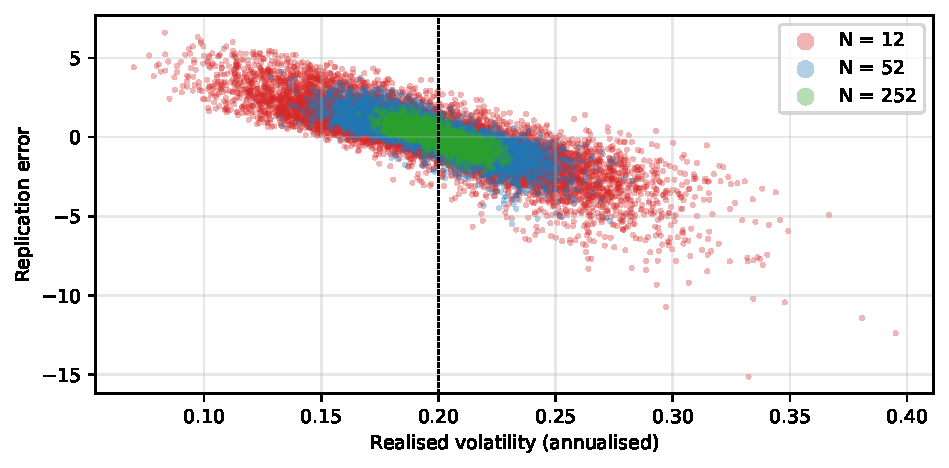
\includegraphics[width=\linewidth]{q1_error_vs_realvol.pdf}
\caption{Replication error against realised volatility.}\label{fig:q1-realvol}
\end{minipage}\hfill
\begin{minipage}[t]{0.49\textwidth}\centering
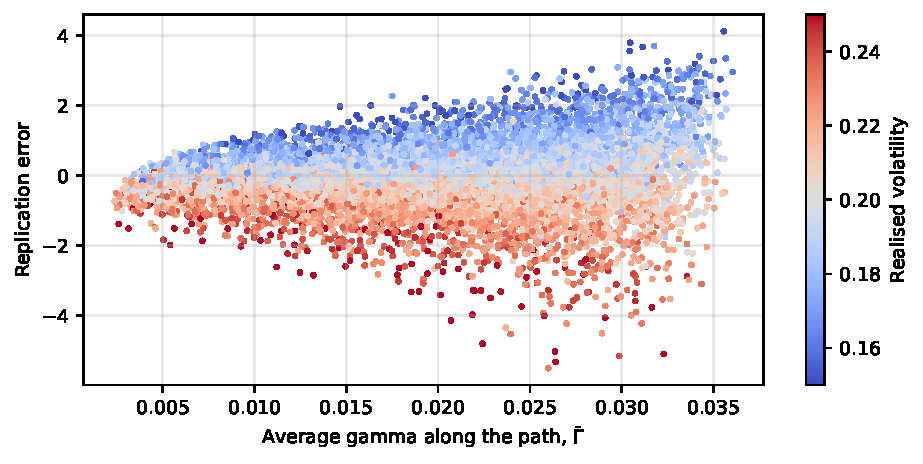
\includegraphics[width=\linewidth]{q1_error_vs_gamma.pdf}
\caption{Replication error against average gamma ($N=52$), coloured by
realised volatility.}\label{fig:q1-gamma}
\end{minipage}
\end{figure}
There is a strong negative relationship: the correlation with realised
variance is about $-0.81$ for every $N$. A second-order (Taylor) expansion
of the hedged position gives
\begin{equation*}
\text{error}\;\approx\;\tfrac12\sum_i \Gamma_i S_i^2
\left(\sigma^2-\sigma_{\text{real},i}^2\right)\Delta t .
\end{equation*}
The option is long gamma and the replicating portfolio is not. The premium
we received pays for $20\%$ volatility. If the stock actually moved more
($\sigma_\text{real}>20\%$), the option is worth more than our portfolio and
the error is negative; if it moved less, we make money. The scatter around
the line is the pure discreteness error, which narrows as $N$ grows.

The plot fans out: the higher the average gamma, the larger the absolute
error. The error standard deviation is $1.30$ for the top quartile of
average gamma against $0.54$ for the bottom quartile. Gamma is the
\emph{size} of the exposure and the volatility surprise
$\sigma^2-\sigma_{\text{real}}^2$ sets its \emph{sign}, as the colours show:
low-volatility (blue) paths sit above zero and high-volatility (red) paths
below. High-gamma paths are those that stay near the strike. Using only the
average gamma, the formula above already has a correlation of $0.87$ with
the simulated error.

\subsection*{1(h) Drift sensitivity}
\restab{q1_drift}{Hedging error for different real-world drifts ($N=52$,
10,000 paths, the same random numbers for every $\mu$).}{tab:q1-drift}
The drift has a \emph{very small} effect. Raising $\mu$ from $2.5\%$ to
$10\%$ moves the mean terminal price by 8 points, yet the mean absolute error
only goes from $0.711$ to $0.699$ and the variance from $0.904$ to $0.884$,
which is the same order as the Monte Carlo noise. Delta hedging removes the
directional exposure, so the expected return of the stock does not enter
the Black--Scholes price or the hedge. The slight improvement at higher
$\mu$ is because the put then ends further out of the money, where gamma
is lower.

%=============================================================================
\section*{Question 2: Time-varying volatility}
%=============================================================================

\subsection*{2(a) A two-period volatility term structure}
\restab{q2_values}{Put values with $S(0)=K=100$, $r=4\%$, $T=1$.}
{tab:q2-termstructure}
A European payoff depends only on the distribution of $S(T)$. That
distribution is lognormal with total variance $\int_0^T\sigma^2(u)\,du$, so
only the average variance counts:
$\bar\sigma^2=\tfrac12(0.04^2)+\tfrac12(0.28^2)=0.0008+0.0392=0.04=0.20^2$.
The two prices are therefore identical ($6.0040$). A Monte Carlo simulation
of the two-period dynamics confirms this within one standard error.

\subsection*{2(b) \texttt{DeltaHedgeTV}}
The stock path uses the \emph{instantaneous} volatility: each step has
variance $\int_t^{t+\Delta t}\sigma^2(u)du$. Pricing and hedging at time $t$
must use the \emph{average volatility over the remaining life},
$\bar\sigma(t)=\sqrt{\int_t^T\sigma^2(u)du/(T-t)}$. This changes as time to
maturity falls. With the low volatility first, $\bar\sigma(t)$ rises from
$20\%$ at $t=0$ to $28\%$ at $t=\tfrac12$ and then stays there. With the
high volatility first, it falls from $20\%$ to $4\%$.
\code{tvhelpers}{Integrated variance and remaining-life average volatility.}
\code{deltahedgetv}{\texttt{DeltaHedgeTV}.}

\subsection*{2(c) Hedging performance with time-varying volatility}
\fig[0.85\textwidth]{q2_error_vs_ST.pdf}{Hedging error against $S(T)$,
$N=52$, 10,000 paths, the same random numbers in all panels.}
{fig:q2-hedge}
\restab{q2_compare}{Hedging error: constant versus time-varying volatility
(4\% then 28\%), 10,000 paths.}{tab:q2-compare}
With the correct $\bar\sigma(t)$ the hedge is still unbiased (mean
$\approx0$), but the error variance almost \emph{doubles} at every $N$
($1.69$ against $0.90$ for $N=52$). Hedging with today's instantaneous
volatility instead gives a large bias and four times the variance
(mean $+0.54$, variance $3.90$ at $N=52$).

\subsection*{2(d) Reversing the volatility structure}
\restab{q2_reversed}{Hedging error when the high-volatility period comes first
(28\% then 4\%), 10,000 paths.}{tab:q2-reversed}

\subsection*{2(e) Comparing the three cases}
\begin{itemize}[leftmargin=*]
\item \textbf{Price.} All three cases have the same total variance, so the
  premium is the same and, with the correct remaining-life volatility, the
  mean hedging error is zero in all three.
\item \textbf{Risk.} Both time-varying cases have roughly twice the error
  variance of the constant case. Each step's error is roughly
  $\tfrac12\Gamma S^2(\Delta S^2/S^2-\sigma_t^2\Delta t)$, whose variance
  grows with $\sigma_t^4$. The total error variance therefore depends on
  $\int\sigma^4\,dt$, not on $\int\sigma^2\,dt$. With constant volatility
  $\sigma^4=0.0016$; for the two-period cases the average
  $\tfrac12(0.04^4+0.28^4)=0.0031$ is $1.92$ times larger, close to the
  observed ratios ($1.84$--$1.88$ for low-first, $1.74$--$1.81$ for
  high-first). The same variance delivered in fewer, larger moves is harder
  to hedge discretely.
\item \textbf{Ordering.} Low-volatility-first is slightly riskier than
  high-volatility-first ($1.69$ against $1.58$ at $N=52$). With the quiet
  period first, the stock is still close to the strike when the volatile
  period starts, and those large moves then happen close to expiry, where
  delta changes fastest for at-the-money paths. With the volatile period
  first, the large moves happen while the option still has a long time to
  run; by the time expiry approaches the stock has usually moved away from
  the strike and barely moves.
\item \textbf{Main lesson.} Using the right volatility matters much more
  than the ordering. The naive hedge with the instantaneous volatility is
  biased ($+0.54$) and has a variance of $3.90$.
\end{itemize}

%=============================================================================
\section*{Question 3: Asian options and the control variate technique}
%=============================================================================

\subsection*{3(a) Pricing an arithmetic average Asian call}
The stock is simulated under the risk-neutral measure. One step goes from
$0$ to $T_0=0.25$, because nothing is averaged before $T_0$. Then 90 daily
steps of $\Delta t=0.25/90$ go to $T=0.5$, and $\bar S$ is the average over
those 90 dates. The price is the mean of the discounted payoffs
$e^{-rT}(\bar S-K)^+$. All paths are generated at once with NumPy.
\code{asianpaths}{Path simulation and arithmetic Asian call pricer.}

\subsection*{3(b) A first price}
For $S(0)=K=100$, $r=4\%$, $\sigma=25\%$ and $P=10{,}000$ paths, the price
is $\mathbf{6.4185}$ with a standard error of $0.0974$. The 95\% confidence
interval is $[6.23,\,6.61]$.

\subsection*{3(c)--(d) Adding the geometric average; variances and covariance}
\code{asianfull}{Arithmetic and geometric Asian calls on the same paths;
returns the five requested numbers.}

\subsection*{3(e) Numerical results}
\restab{q3_results}{$S(0)=K=100$, $r=5\%$, $q=1\%$, $\sigma=30\%$, $T=0.5$,
$T_0=0.25$, 90 days, $P=5{,}000$. Variances and covariance are per path
for the discounted payoffs.}{tab:q3-results}
The two payoffs have almost the same variance and a covariance close to
both, so their correlation is close to one. The geometric average is always
below the arithmetic one, so the geometric call is the cheaper option.

\subsection*{3(f) The control variate estimate}
We read ``$T_0=0$'' as averaging that starts today and runs daily (180 days)
to expiry. The second row of Table~\ref{tab:q3-cv} applies the same method
to the original contract with $T_0=0.25$. The discretely sampled geometric
average is exactly lognormal, so its price follows from a Black formula
(Code~\ref{lst:geo}). The best (minimum-variance) estimator is
\begin{equation*}
\hat A_{\text{CV}}=\bar A-\beta\left(\bar G-G^{\text{exact}}\right),\qquad
\beta=\frac{\operatorname{Cov}(A,G)}{\operatorname{Var}(G)},\qquad
\operatorname{Var}(\hat A_{\text{CV}})=\frac{\operatorname{Var}(A)
(1-\rho^2)}{P}.
\end{equation*}
\restab{q3_cv}{Control variate results ($P=5{,}000$). K--V is the
continuous-averaging Kemna--Vorst formula from the lecture.}{tab:q3-cv}
The best estimate of the arithmetic Asian price is $\mathbf{5.3255}$
(standard error $0.0032$) for $T_0=0$, and $7.5629$ ($0.0022$) for the
original contract. The control variate cuts the standard error by a factor
of 35 to 75. The geometric price must be the \emph{discrete} formula: the
continuous Kemna--Vorst value differs by about $0.02$, which would bias the
estimate.
\lstinputlisting[linerange=geoexact_start-geoexact_end, label=lst:geo,
caption={Exact discrete geometric Asian price and delta, and the control
variate estimator.}]{ad_coursework_code.py}

\subsection*{3(g) Paths needed with the control variate}
The variance of an estimate is the per-path variance divided by $P$.
Matching the variance of a plain simulation with $P=10{,}000$ paths
therefore requires
$P_{\text{CV}}=10{,}000\cdot\operatorname{Var}_{\text{CV}}/
\operatorname{Var}_{\text{plain}}=10{,}000\,(1-\rho^2)$.
\restab{q3_paths}{Per-path variances and the equivalent number of paths
(estimated with 10,000 paths).}{tab:q3-paths}
Because $\rho>0.999$, in theory only a handful of paths (2--8) give the same
precision as 10,000 plain paths. In practice you still need a few hundred
paths to estimate $\beta$ reliably and for the normal approximation to hold.
Even so, the saving is a factor of more than 1,000.

%=============================================================================
\section*{Question 4: The delta of the Asian option}
%=============================================================================
We use the contract from 3(e): $S(0)=K=100$, $r=5\%$, $q=1\%$, $\sigma=30\%$,
$T=0.5$, averaging daily over the last 90 days, $P=10{,}000$.

\subsection*{4(a) Finite-difference delta}
\code{fddelta}{Forward finite-difference delta.}
\begin{figure}[H]
\begin{minipage}[c]{0.52\textwidth}\centering
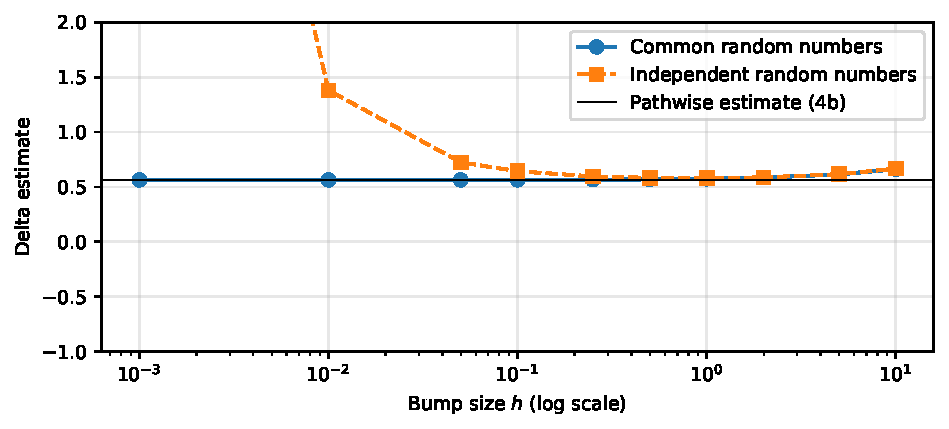
\includegraphics[width=\linewidth]{q4_fd_delta.pdf}
\caption{Finite-difference delta against the bump size $h$.}\label{fig:q4-fd}
\end{minipage}\hfill
\begin{minipage}[c]{0.45\textwidth}\centering\scriptsize
\captionof{table}{Finite-difference delta estimates.}\label{tab:q4-fd}
\begin{tabular}{rrr}
\toprule
$h$ & Common RN & Independent RN \\
\midrule
0.0010 & 0.5637 & 8.7625 \\
0.0100 & 0.5638 & 1.3798 \\
0.0500 & 0.5640 & 0.7239 \\
0.1000 & 0.5645 & 0.6427 \\
0.2500 & 0.5658 & 0.5955 \\
0.5000 & 0.5685 & 0.5824 \\
1.0000 & 0.5743 & 0.5799 \\
2.0000 & 0.5843 & 0.5867 \\
5.0000 & 0.6141 & 0.6159 \\
10.0000 & 0.6615 & 0.6660 \\
\bottomrule
\end{tabular}

\end{minipage}
\end{figure}
We reuse \emph{exactly the same random numbers}, through the same seed and
therefore the same normal draws, for $f(S_0)$ and $f(S_0+h)$ (common random
numbers). Every simulated price is proportional to $S_0$, so the bumped
paths are the base paths scaled by $(1+h/S_0)$. The Monte Carlo noise then
cancels in the difference, and the estimate is stable and converges to the
pathwise value $0.5637$ as $h\to0$. For large $h$ the forward difference is
biased upwards by about $\tfrac12\Gamma h$. With \emph{independent} random
numbers the noise of the two prices is divided by $h$ and explodes ($8.76$
for $h=0.001$). A bump of about $0.01$--$0.1$ with common random numbers is
a good choice.

\subsection*{4(b) Pathwise delta}
\code{pathwise}{Pathwise delta estimator (no control variate).}
Delta is estimated as the sample mean of
$e^{-rT}\mathbb I(\bar S>K)\bar S/S(0)$ over the paths. The pathwise delta
is $\mathbf{0.5637}$ with a standard error of $0.0057$. It needs no bump and
only one simulation.

\subsection*{4(c) Control variate for the delta}
The control is the pathwise delta of the geometric option,
$e^{-rT}\mathbb I(G>K)G/S(0)$. Its expectation is known analytically:
$e^{-rT}\,\mathbb E[G]\,\Phi(d_1)/S(0)$ (Code~\ref{lst:geo}).
\restab{q4_cv}{Plain versus control variate estimates, $P=10{,}000$.
``Var.\ reduction'' is $1/(1-\rho^2)$.}{tab:q4-cv}
The control variate still helps for the delta: the standard error falls from
$0.0057$ to $0.0006$, equivalent to about 80 times more paths. It is,
however, \emph{far less effective} than for the price, where the variance
falls by a factor of about 6,500. The delta payoff contains the indicator
$\mathbb I(\bar S>K)$, which jumps. On the $0.4\%$ of paths where the
arithmetic and geometric averages fall on opposite sides of the strike, one
indicator is 1 and the other is 0. That drops the correlation from $0.9999$
to $0.994$, and since the variance reduction is $1/(1-\rho^2)$, it is very
sensitive to how close $\rho$ is to one.

\end{document}
